\noindent

\includegraphics[height=1.25cm]{images/pictograms/benchmark}

\includegraphics[height=1.25cm]{images/pictograms/FEM}

\includegraphics[height=1.25cm]{images/pictograms/wave}

%%%%%%%%%%%%%%%%%%%%%%%%%%%%%%%%%%%%%%%%%%%%%%%%%%%%%%%%%%%%%%%%%%%%%%%%%%%%%%%%%%%%%%%%%%%%%%%%%%%

\begin{flushright} {\tiny {\color{gray} python\_codes/fieldstone\_165/text.tex}} \end{flushright}

%\lstinputlisting[language=bash,basicstyle=\small]{python_codes/template_keywords.key}

\par\noindent\rule{\textwidth}{0.4pt}

\begin{center}
\inpython
{\small Code: \url{https://github.com/cedrict/fieldstone/tree/master/python_codes/fieldstone_165}}
\end{center}

\par\noindent\rule{\textwidth}{0.4pt}

%%%%%%%%%%%%%%%%%%%%%%%%%%%%%%%%%%%%%%%%%%%%%%%%%%%%%%%%%%%%%%%%%%%%%%%%%%%%%%%%%%%%%%%%%%%%%%%%%%%

This \stone solves the 2d wave equation using 1st- and 2nd-order finite elements. 
The theory is presented in Chapter~\ref{MMM-fem_waveq}.
The implementation follows \stone~164 although in this case 
a more generic approach is taken: the elemental matrices and rhs vectors for 
each element are computed by means of numerical quadrature.
The code is quite close to \stone~43 which solves the advection-diffusion equation in 2D.
Note that visualisation now relies on vtu files for Paraview.  

Various experiments are carried out:
\begin{itemize}
\item Experiment \# 1:
The domain is a square of size 2, the time step is $dt=0.01$
and the wave speed is set to $c=1$. We have
\[
u(x,y,t=0)=\cos\left[ (x-1)\frac{\pi}{2}\right] \cos\left[ (y-1)\frac{\pi}{2} \right]
\]
and 
\[
\dot{u}(x,y,0)=0
\]
\item Experiment \#2:
Same as experiment \#1, but with
\[
u(x,y,t=0)=\left( \cos\left[ (x-0.25) 2\pi\right] \cos\left[ (y-0.25)2 \pi \right] \right)^2
\]
if $x,y \le 0.5$ and zero otherwise.

\item Experiment \#3:
Same as Experiment \#2, but an additional condition $u=0$ is set for the nodes with $x=L_x/2$
and $y<L_y/2$.

\end{itemize}

Note that although in what follows the values of $u$ is set to zero 
on all four boundaries it can also not be fixed on the boundary(ies)
and therefore yields an implicit Neumann boundary condition $du/dn=0$.

%==============================================
\section*{Results (Experiment \# 1)}

\begin{center}
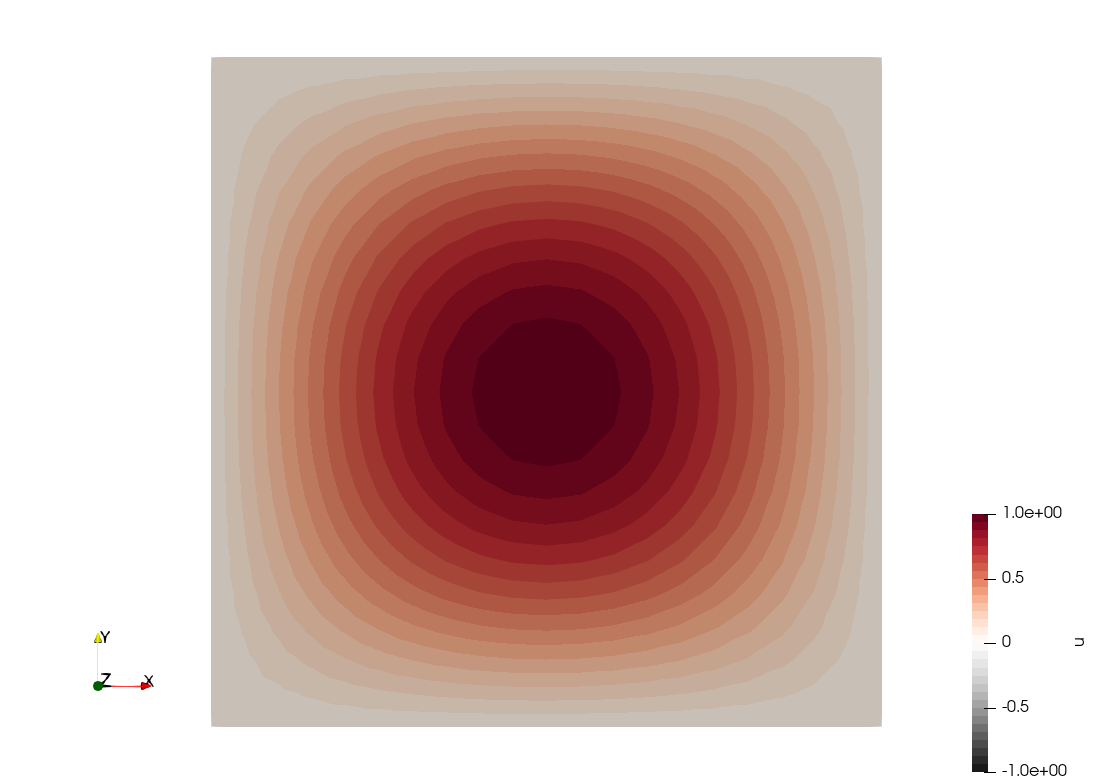
\includegraphics[width=4cm]{python_codes/fieldstone_165/results1/uu0000.png}
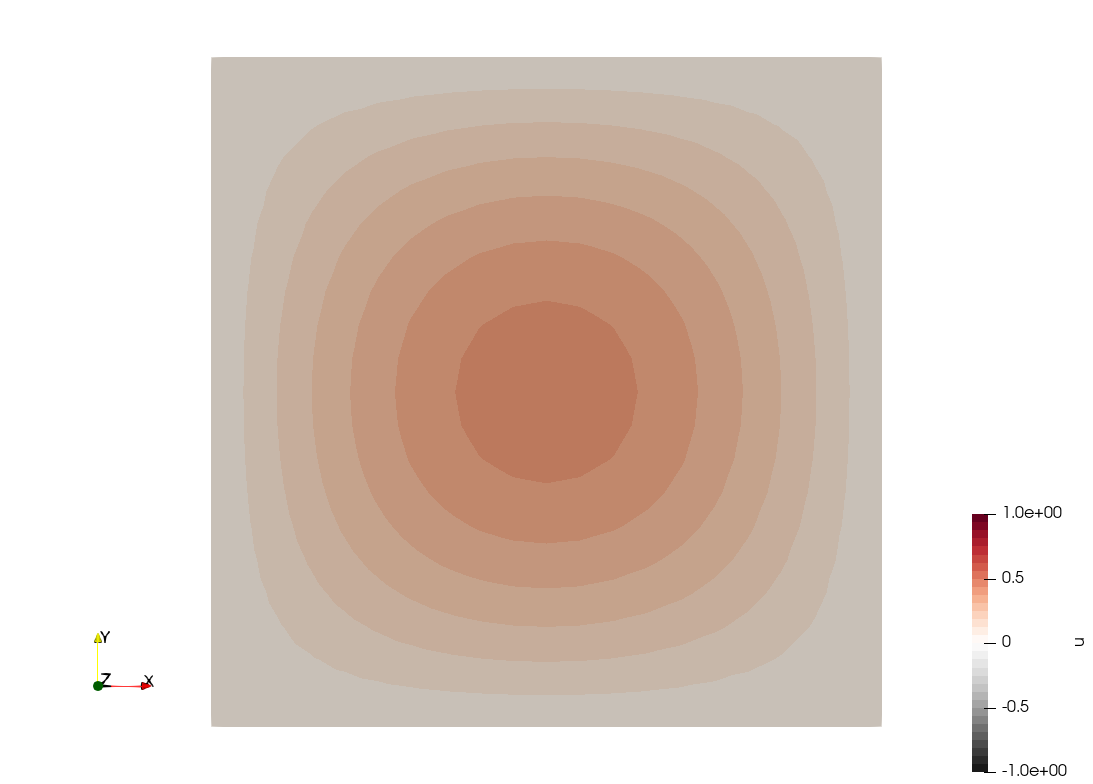
\includegraphics[width=4cm]{python_codes/fieldstone_165/results1/uu0050.png}
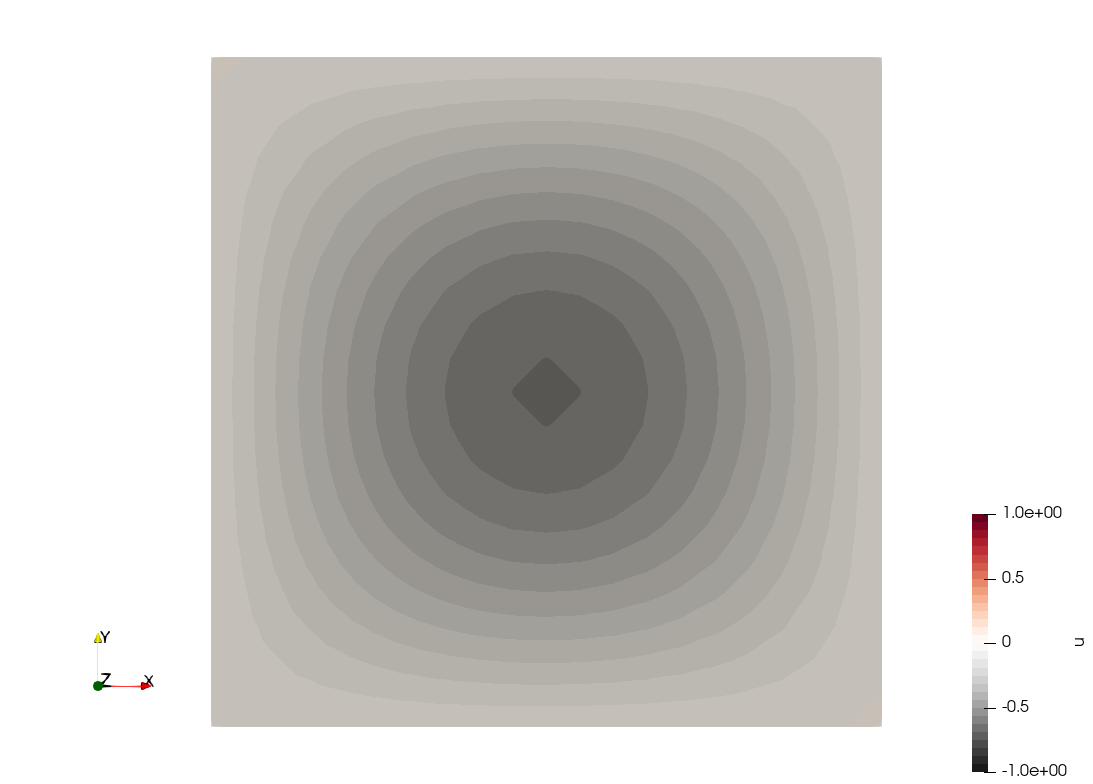
\includegraphics[width=4cm]{python_codes/fieldstone_165/results1/uu0100.png}\\
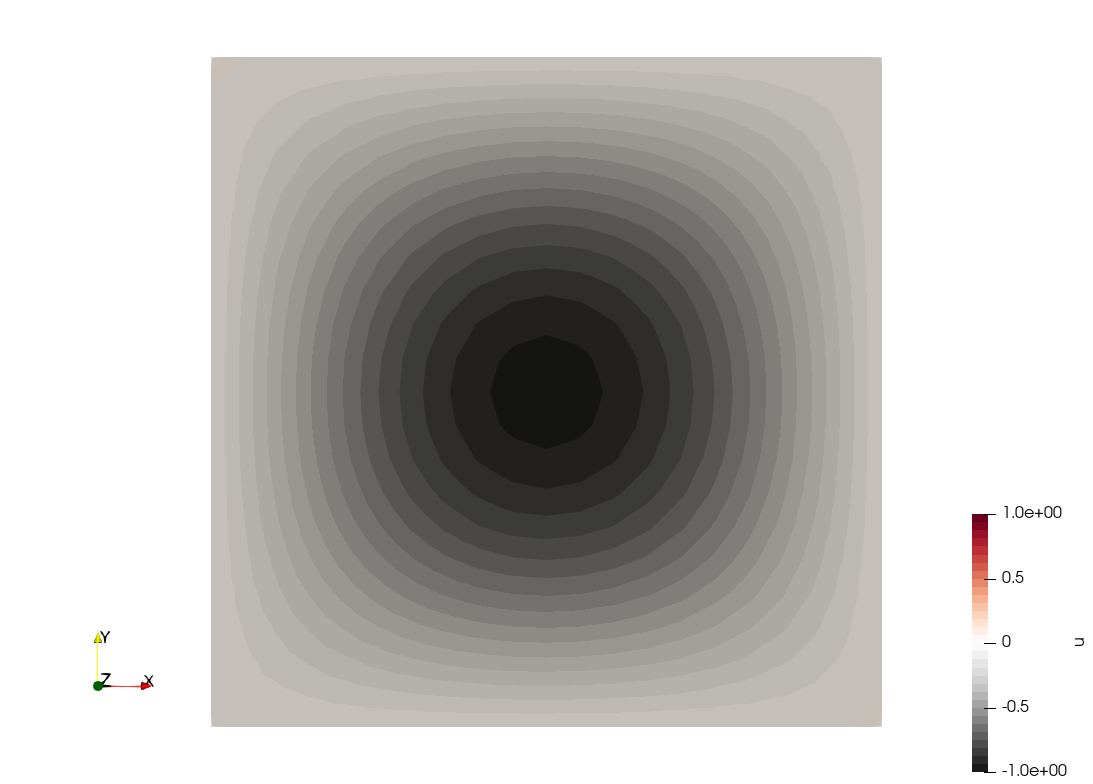
\includegraphics[width=4cm]{python_codes/fieldstone_165/results1/uu0150.png}
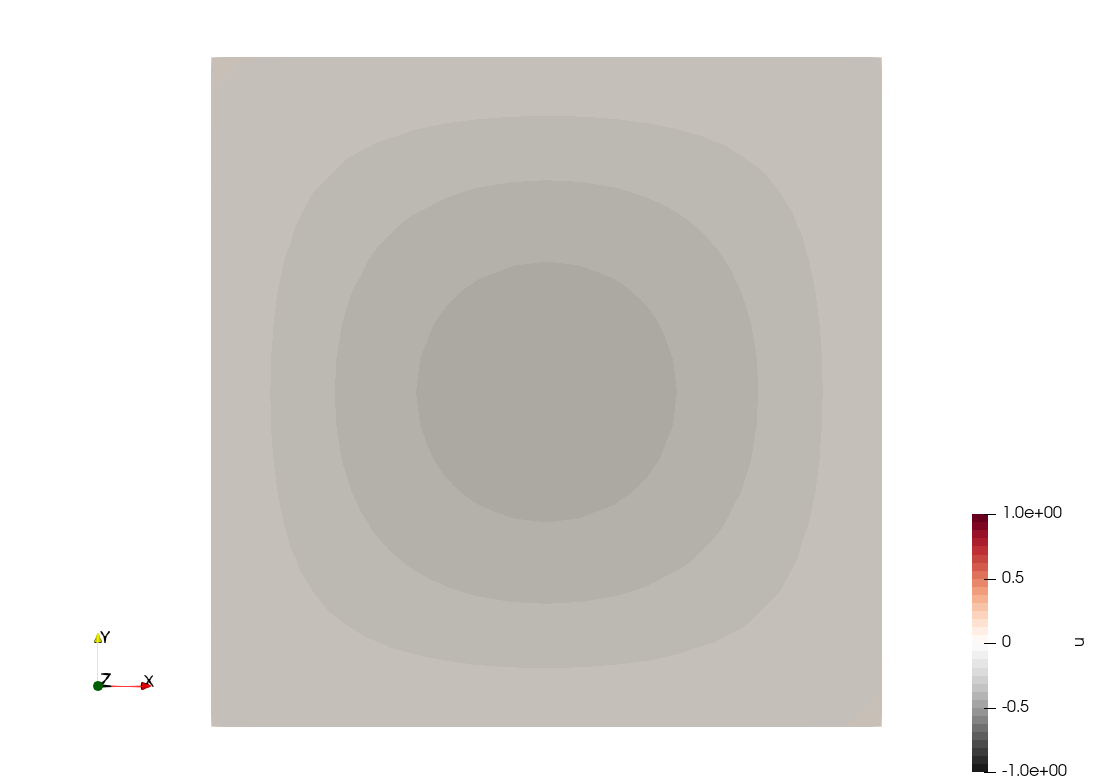
\includegraphics[width=4cm]{python_codes/fieldstone_165/results1/uu0200.png}
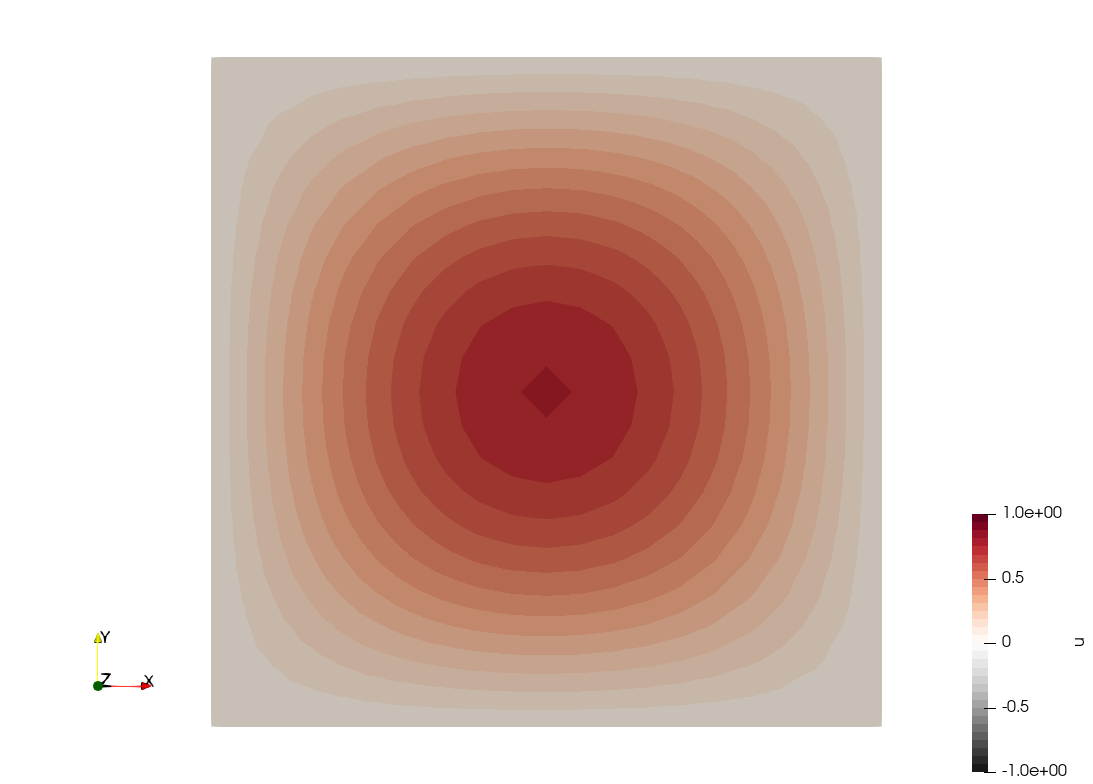
\includegraphics[width=4cm]{python_codes/fieldstone_165/results1/uu0249.png}
\end{center}

\begin{center}
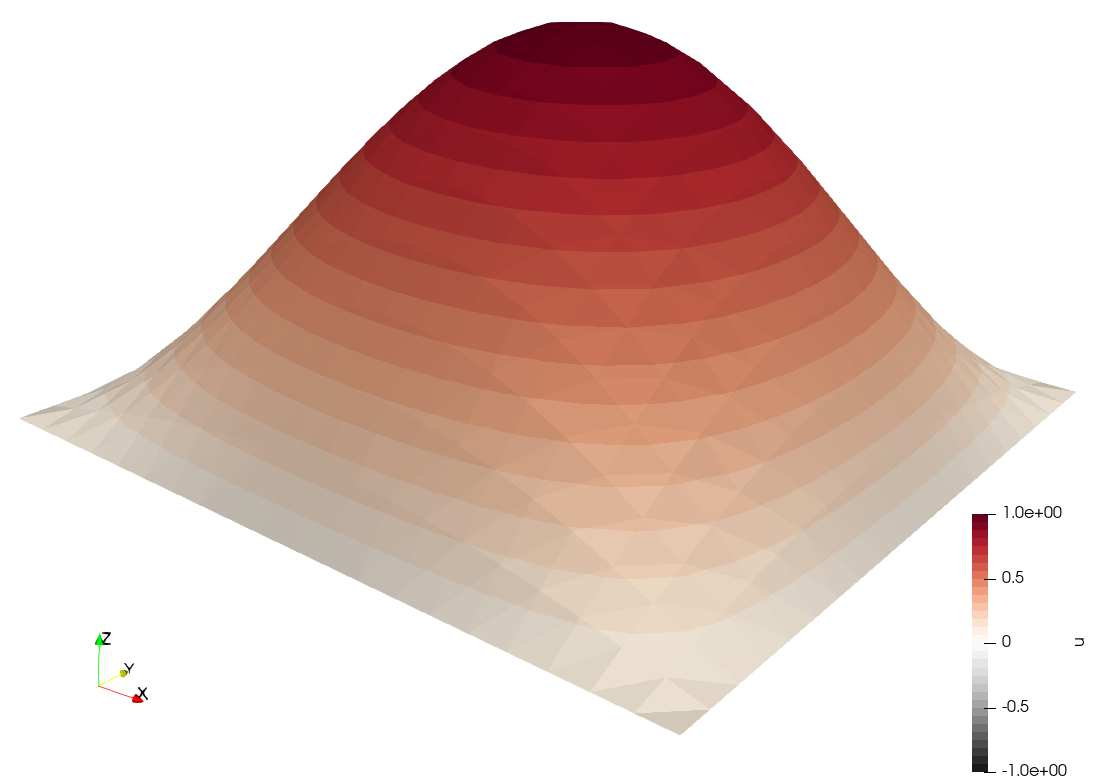
\includegraphics[width=4cm]{python_codes/fieldstone_165/results1/uuu0000.png}
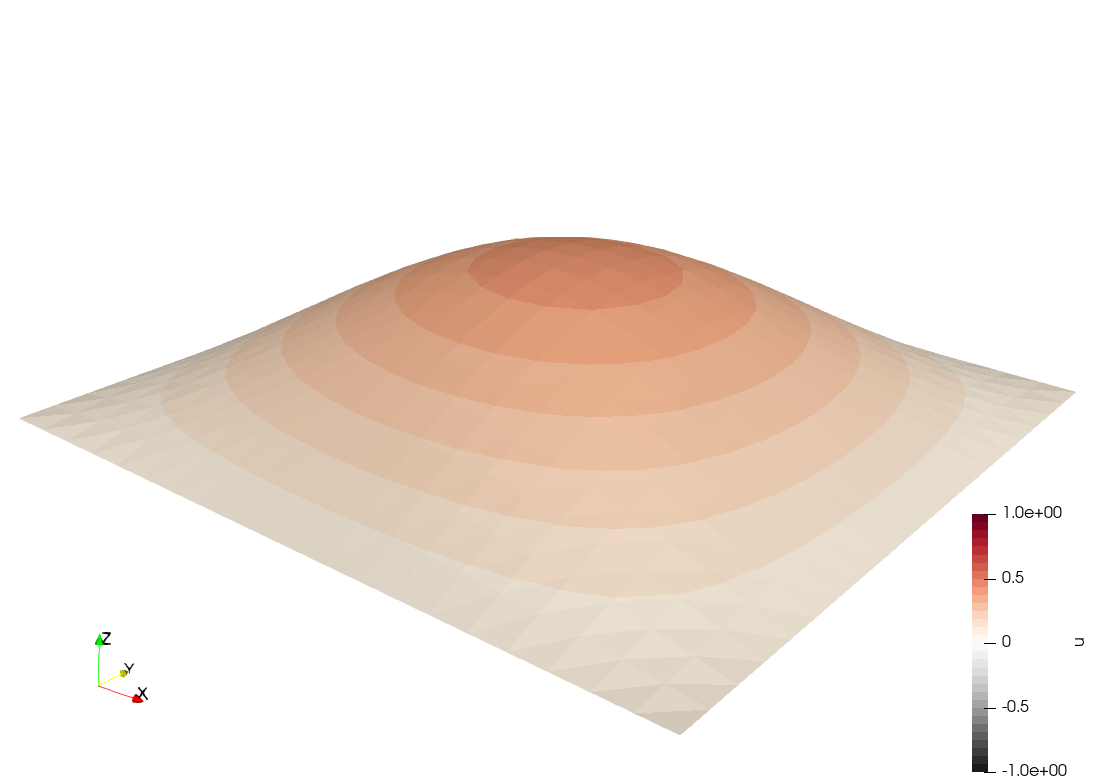
\includegraphics[width=4cm]{python_codes/fieldstone_165/results1/uuu0050.png}
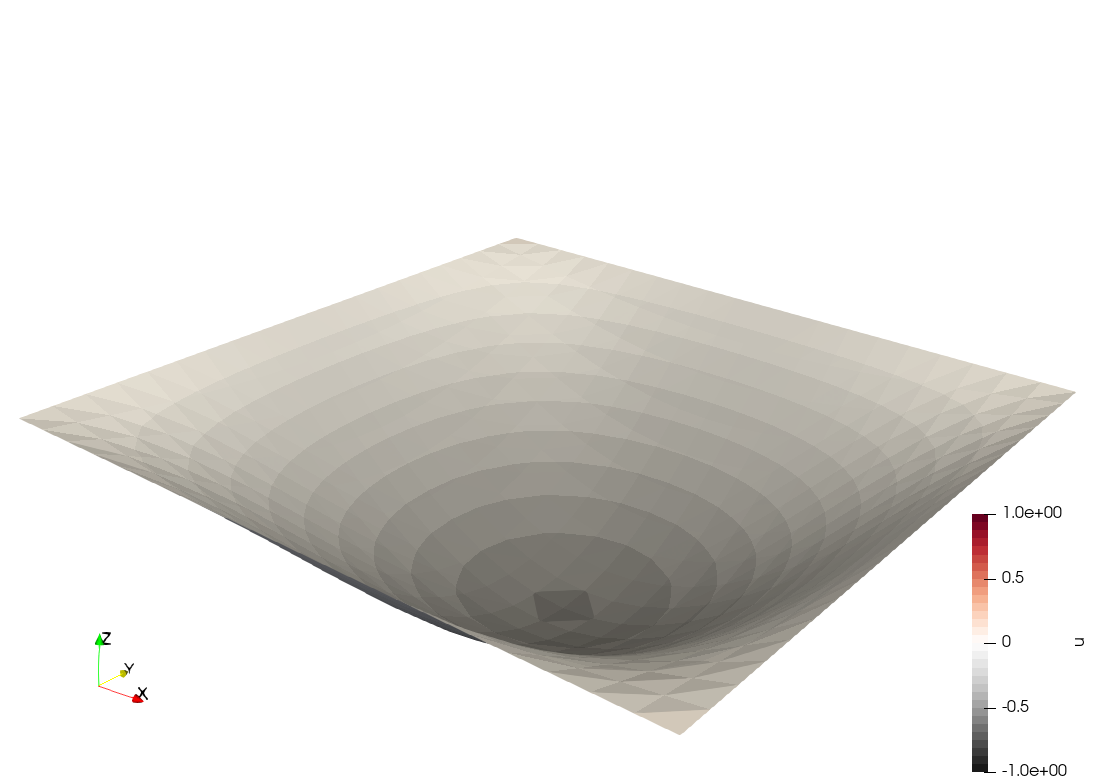
\includegraphics[width=4cm]{python_codes/fieldstone_165/results1/uuu0100.png}\\
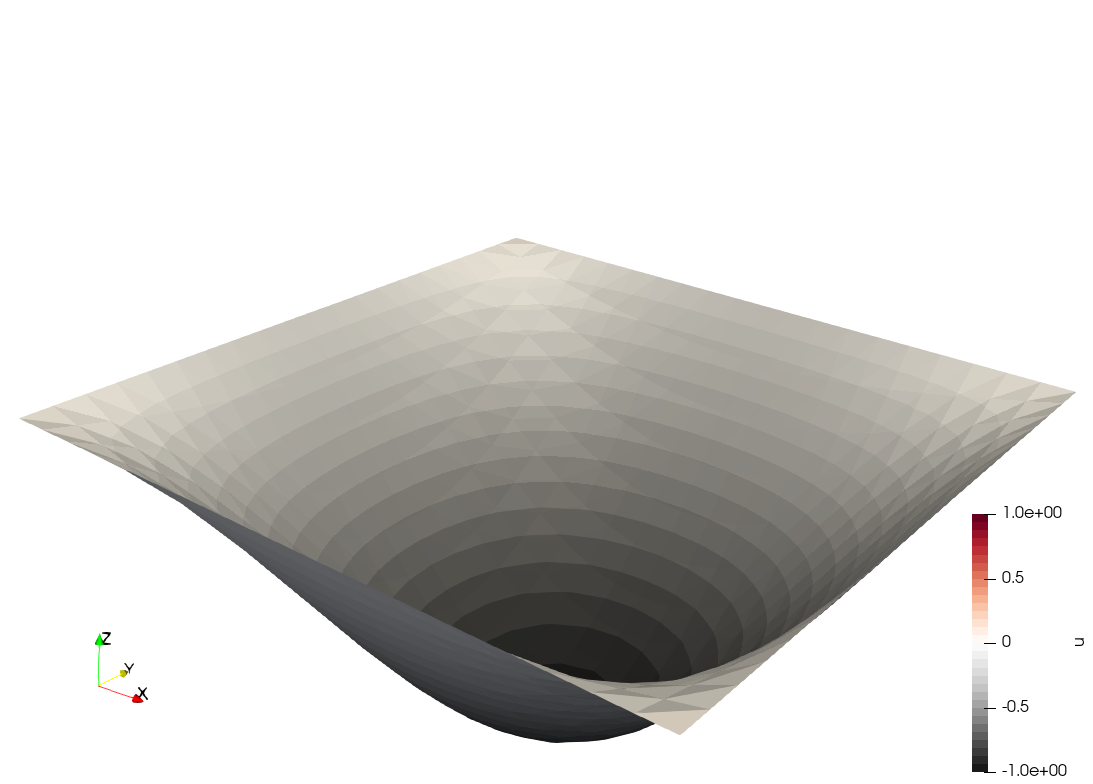
\includegraphics[width=4cm]{python_codes/fieldstone_165/results1/uuu0150.png}
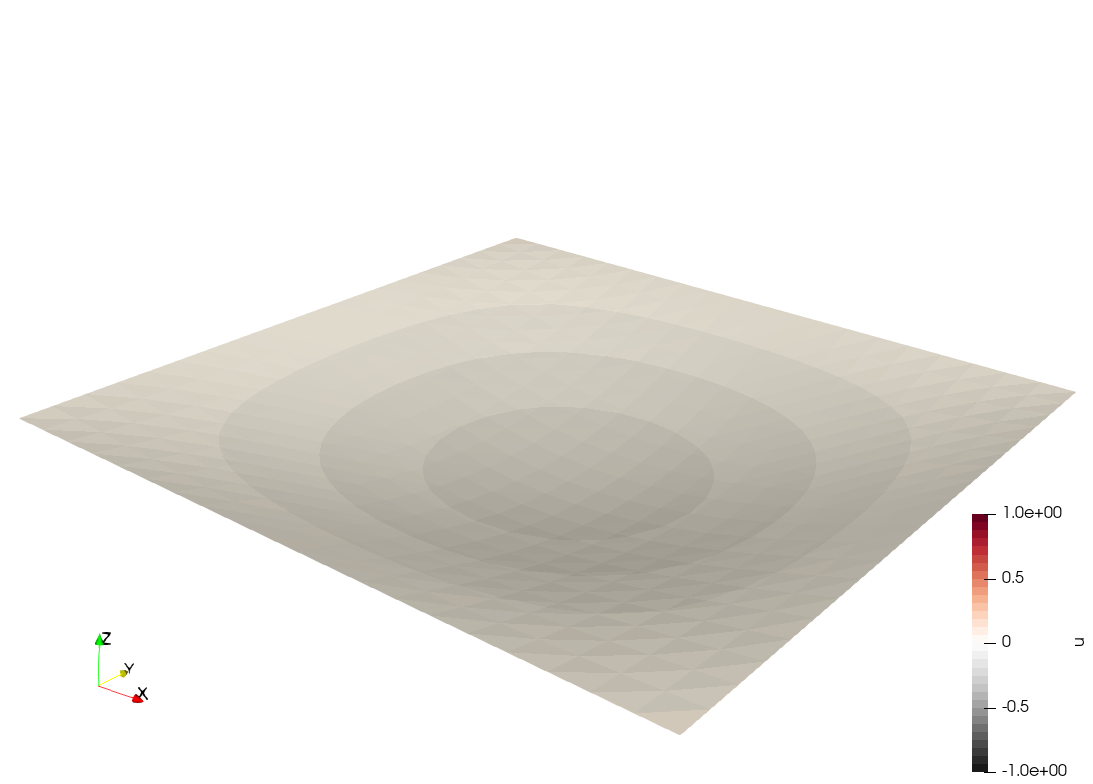
\includegraphics[width=4cm]{python_codes/fieldstone_165/results1/uuu0200.png}
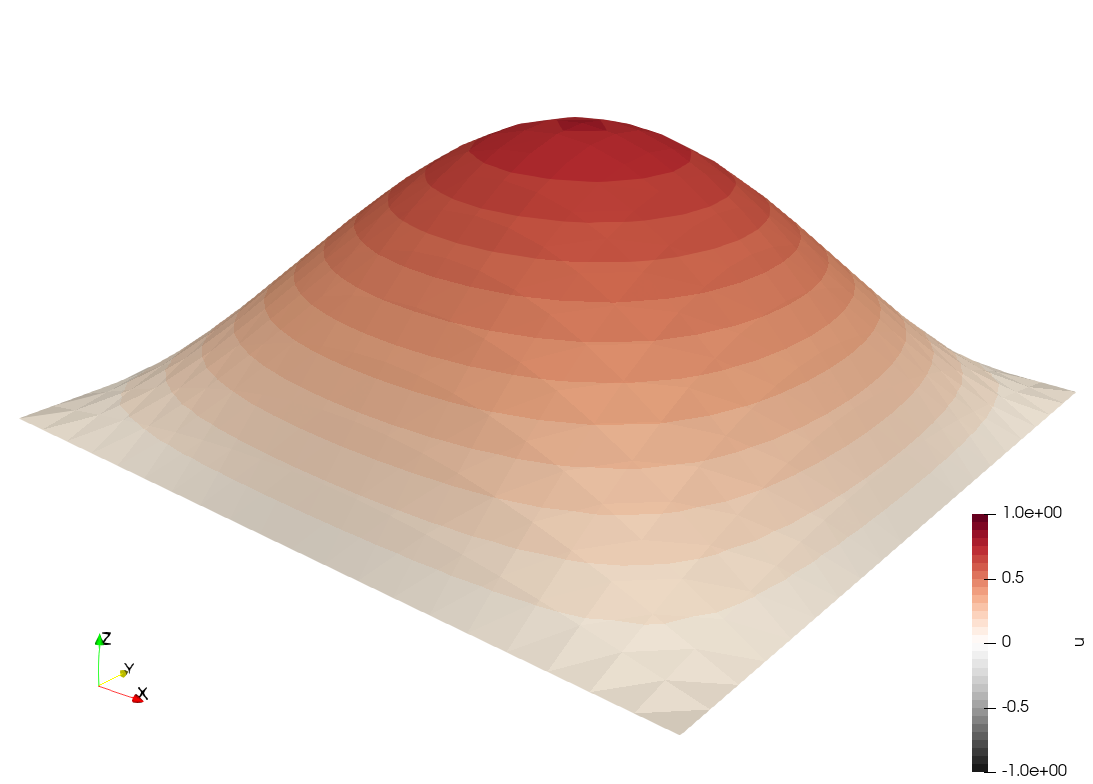
\includegraphics[width=4cm]{python_codes/fieldstone_165/results1/uuu0249.png}
\end{center}







%==============================================
\section*{Results (Experiment \# 2)}

The resolution is set to $64x64$ elements and the simulation 
is ran for 300 time steps. Obtained with 1st order elements. 

\begin{center}
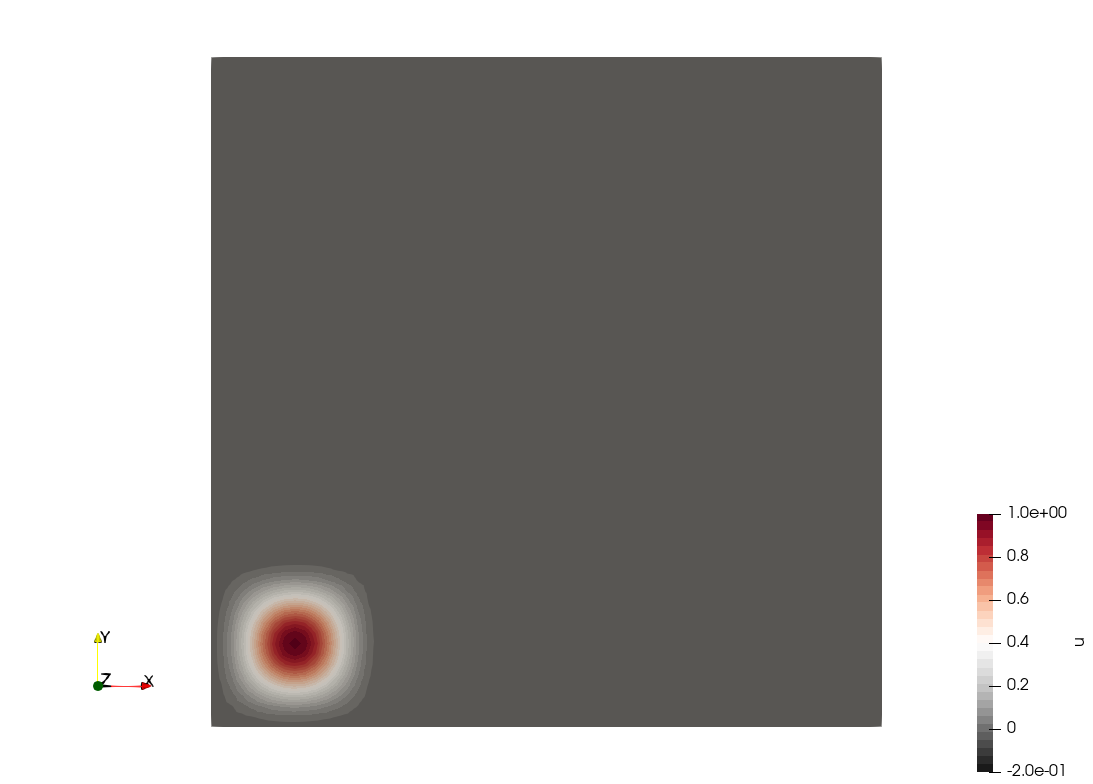
\includegraphics[width=4cm]{python_codes/fieldstone_165/results2/uu0000.png}
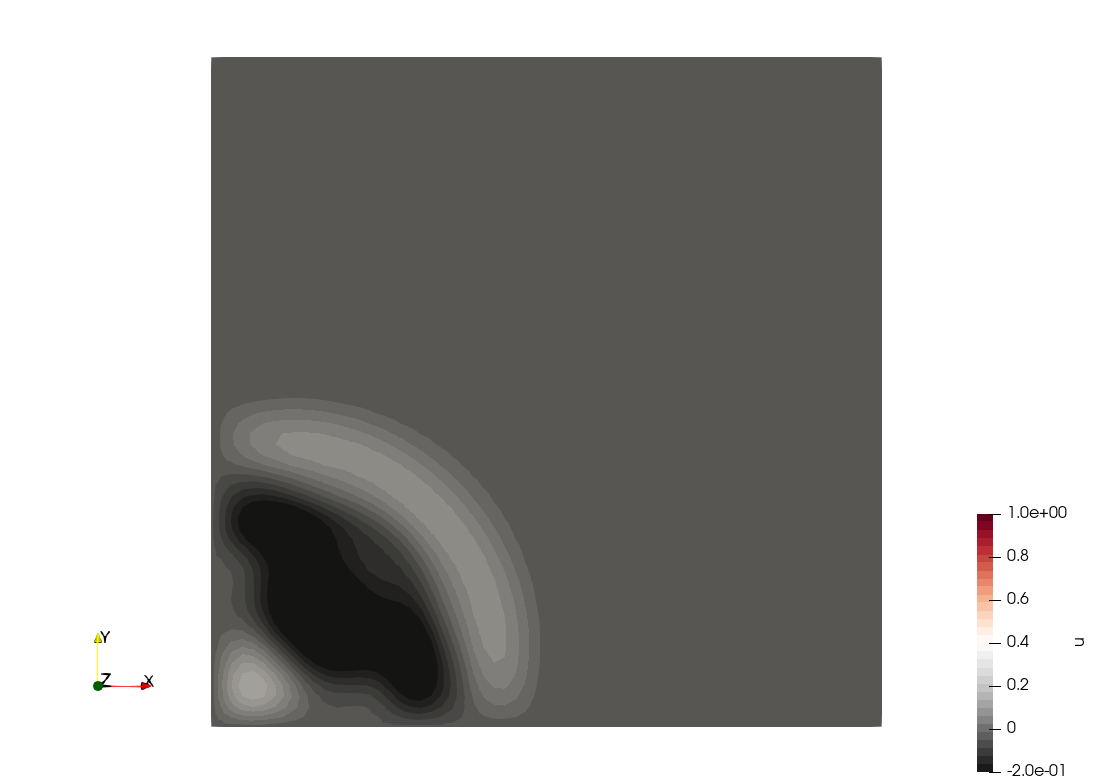
\includegraphics[width=4cm]{python_codes/fieldstone_165/results2/uu0050.png}
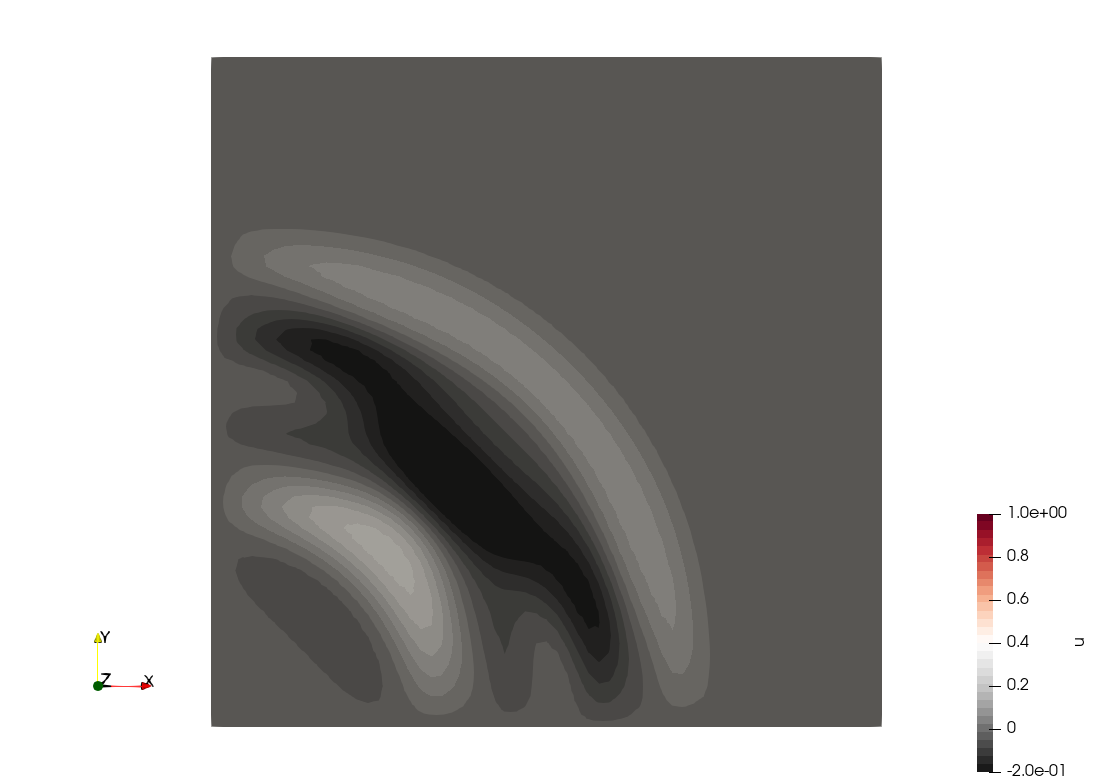
\includegraphics[width=4cm]{python_codes/fieldstone_165/results2/uu0100.png}
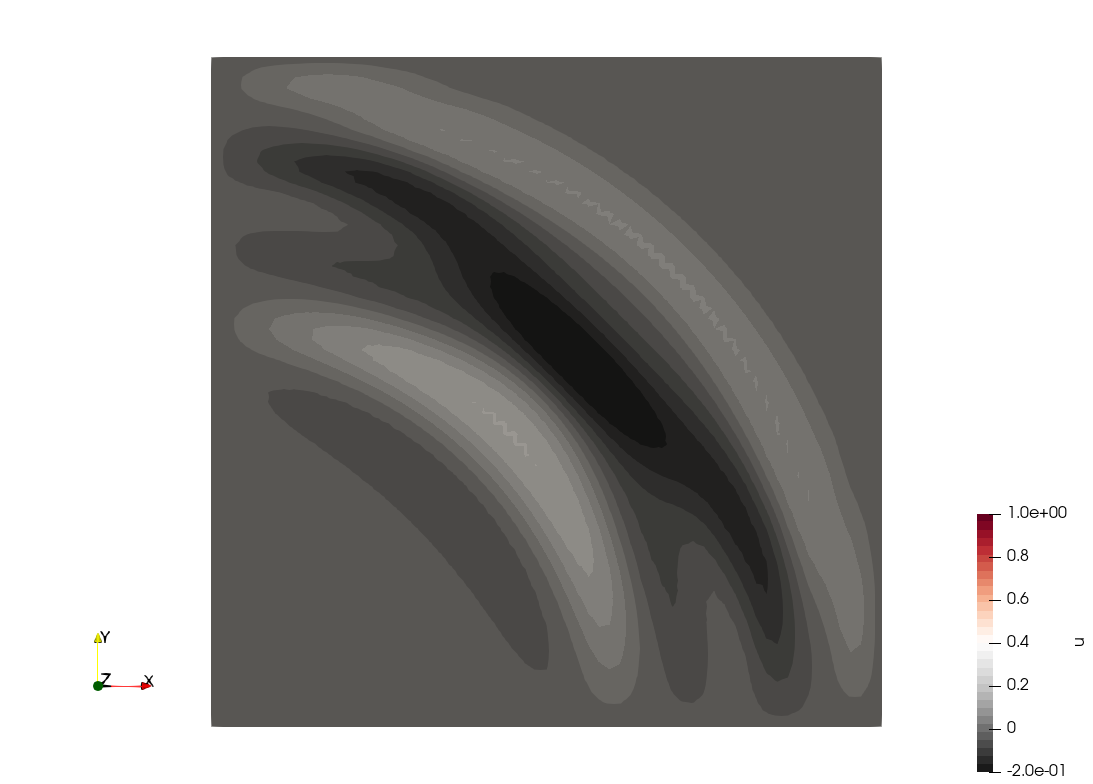
\includegraphics[width=4cm]{python_codes/fieldstone_165/results2/uu0150.png}\\
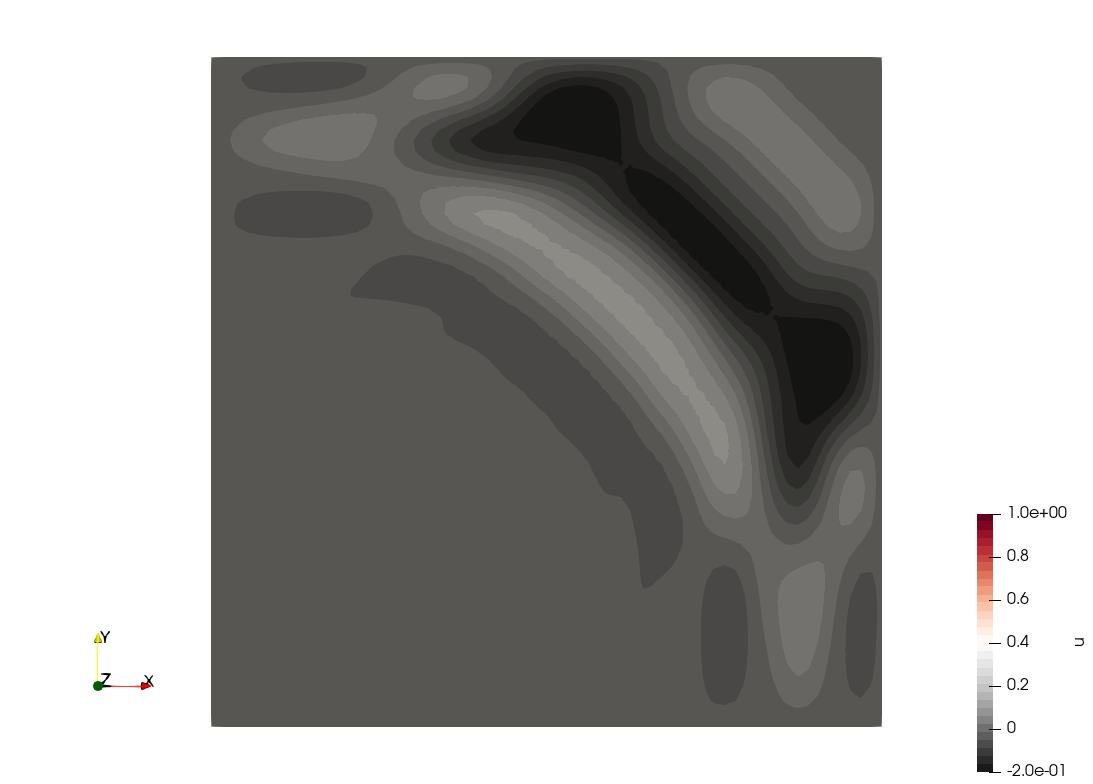
\includegraphics[width=4cm]{python_codes/fieldstone_165/results2/uu0200.png}
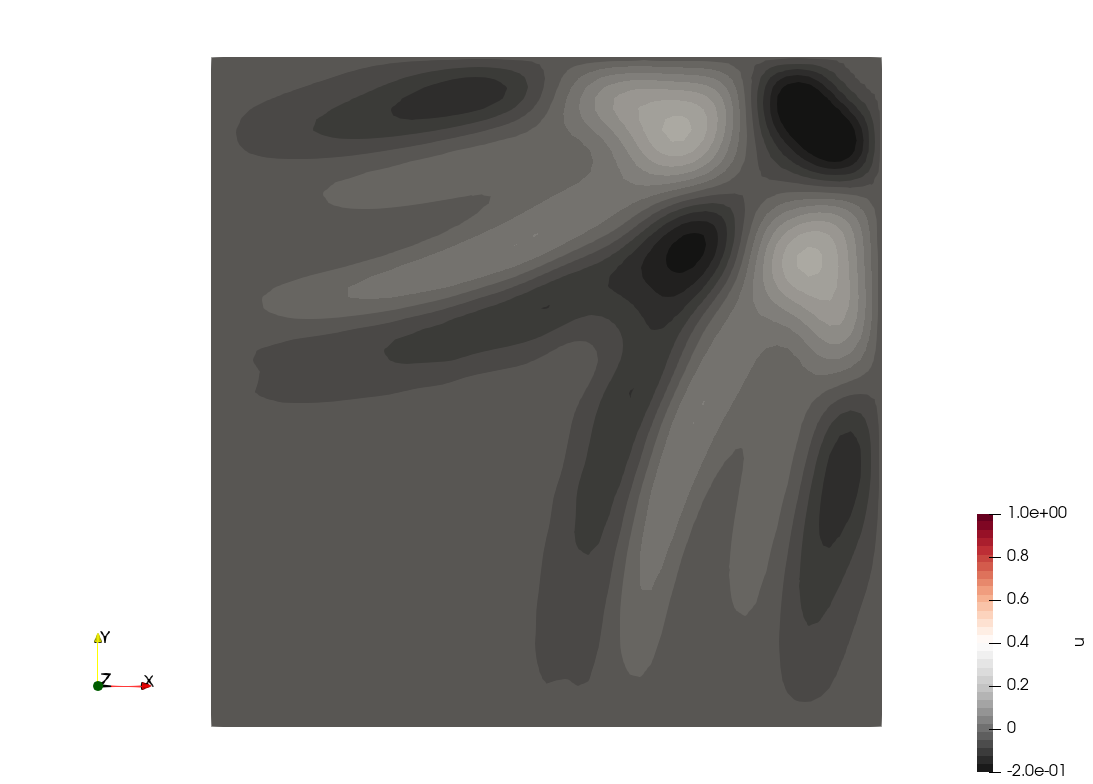
\includegraphics[width=4cm]{python_codes/fieldstone_165/results2/uu0250.png}
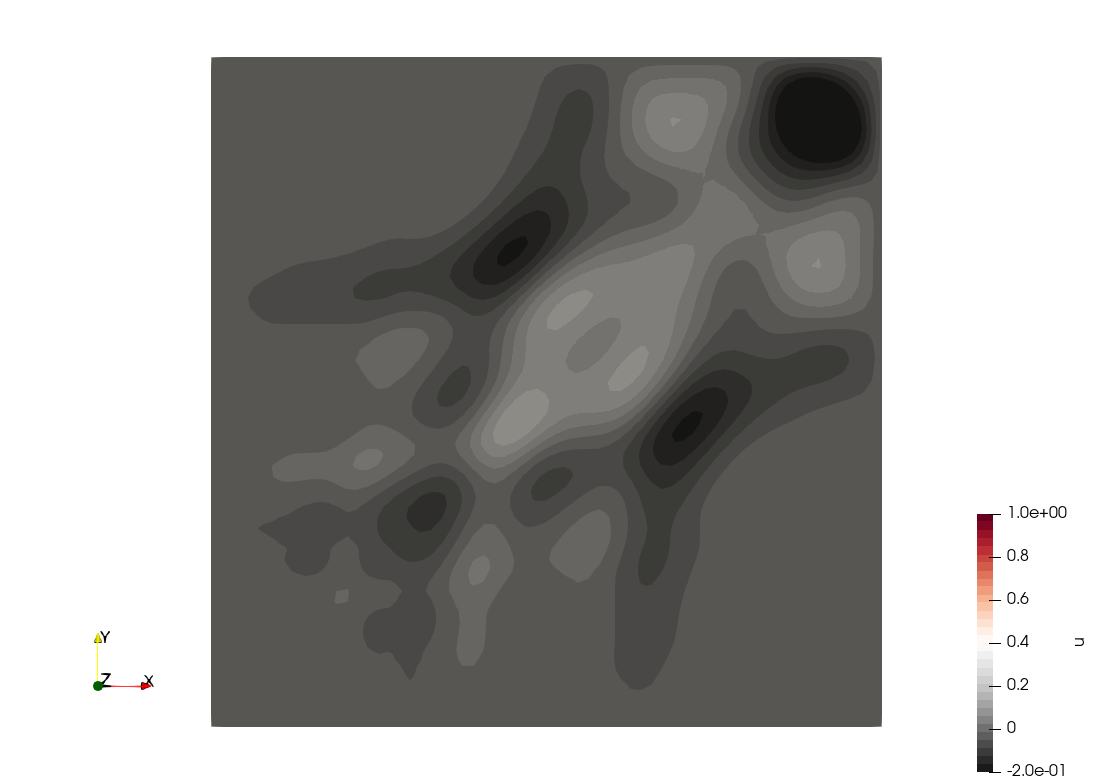
\includegraphics[width=4cm]{python_codes/fieldstone_165/results2/uu0299.png}
\end{center}

\begin{center}
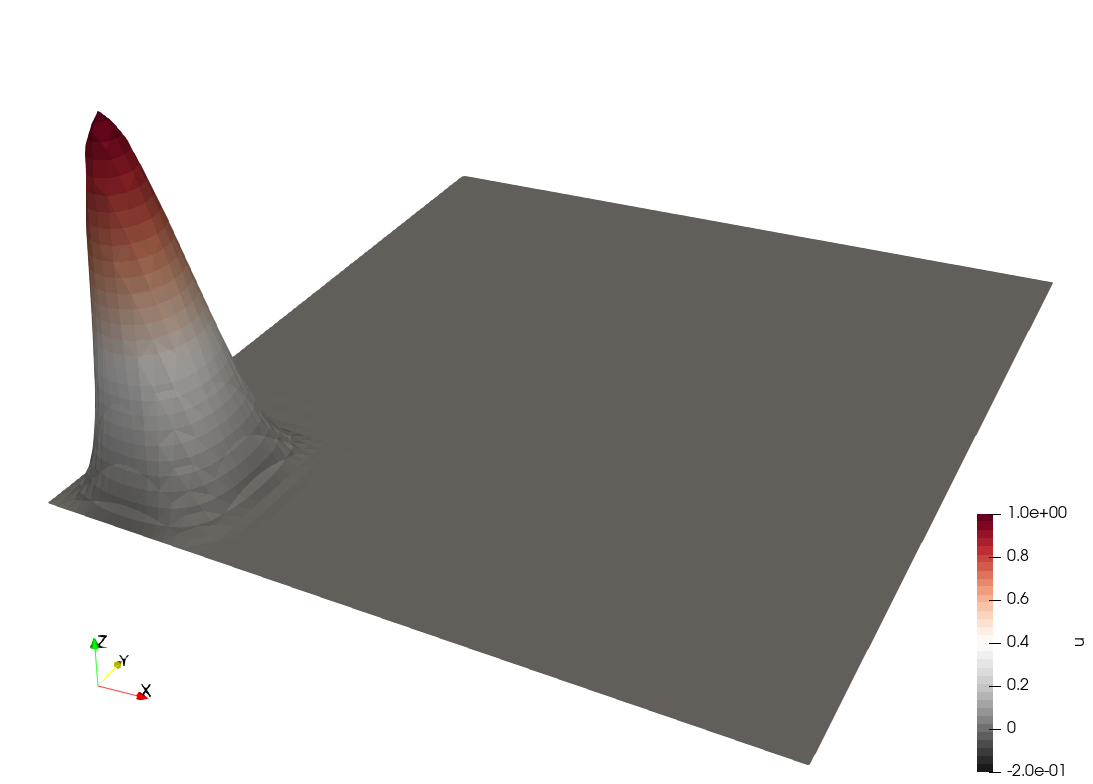
\includegraphics[width=4cm]{python_codes/fieldstone_165/results2/uuu0000.png}
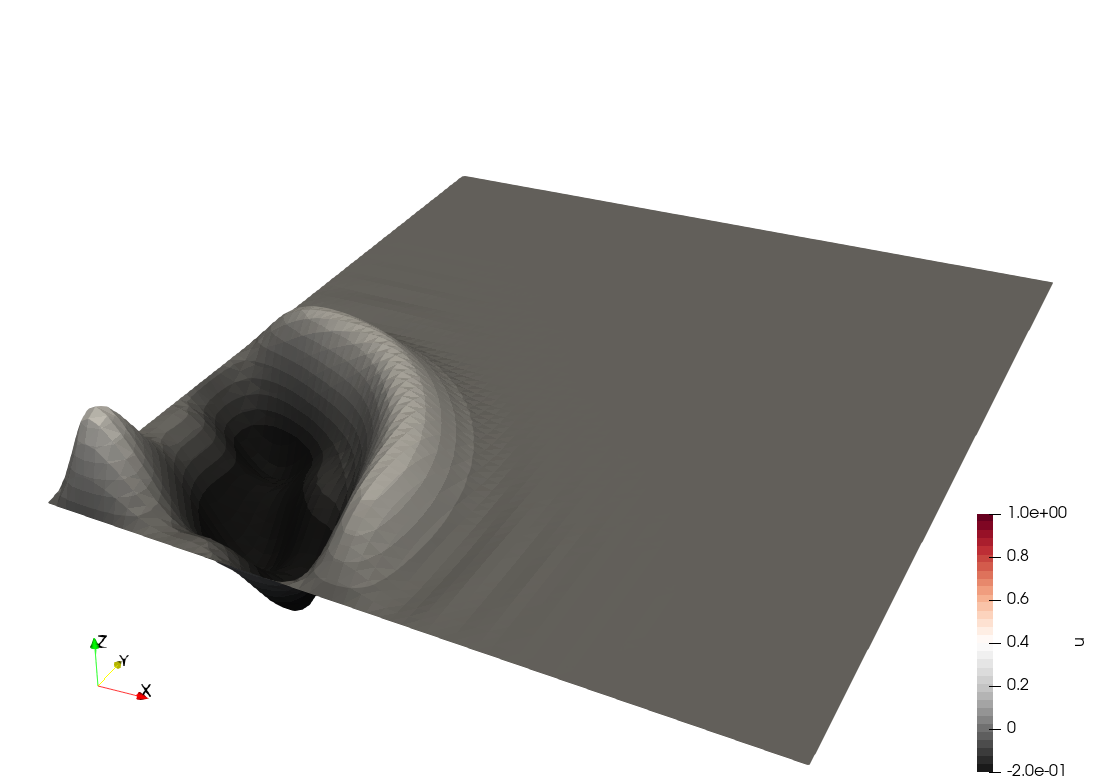
\includegraphics[width=4cm]{python_codes/fieldstone_165/results2/uuu0050.png}
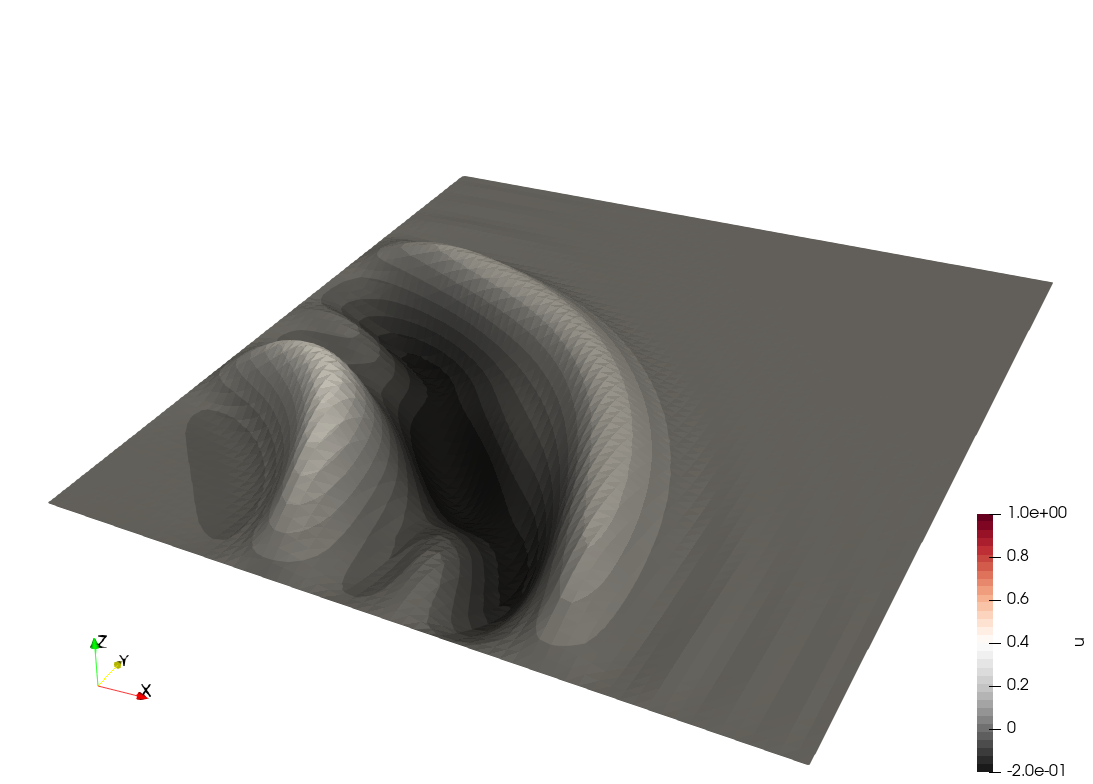
\includegraphics[width=4cm]{python_codes/fieldstone_165/results2/uuu0100.png}
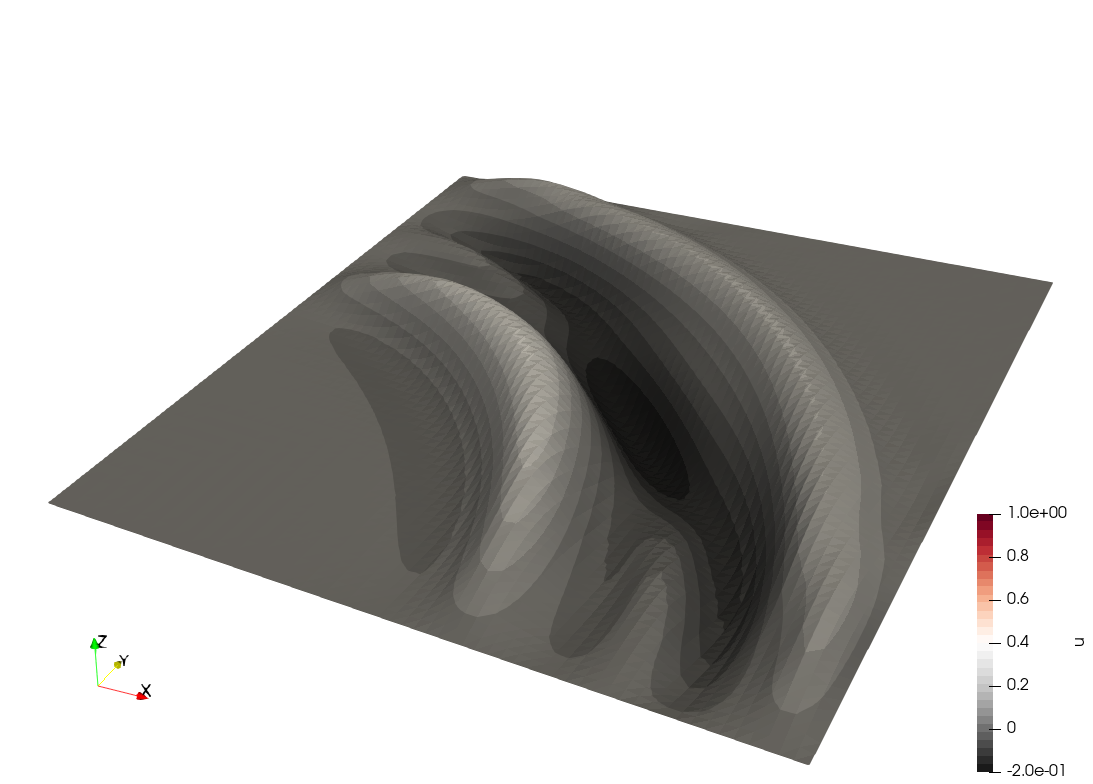
\includegraphics[width=4cm]{python_codes/fieldstone_165/results2/uuu0150.png}\\
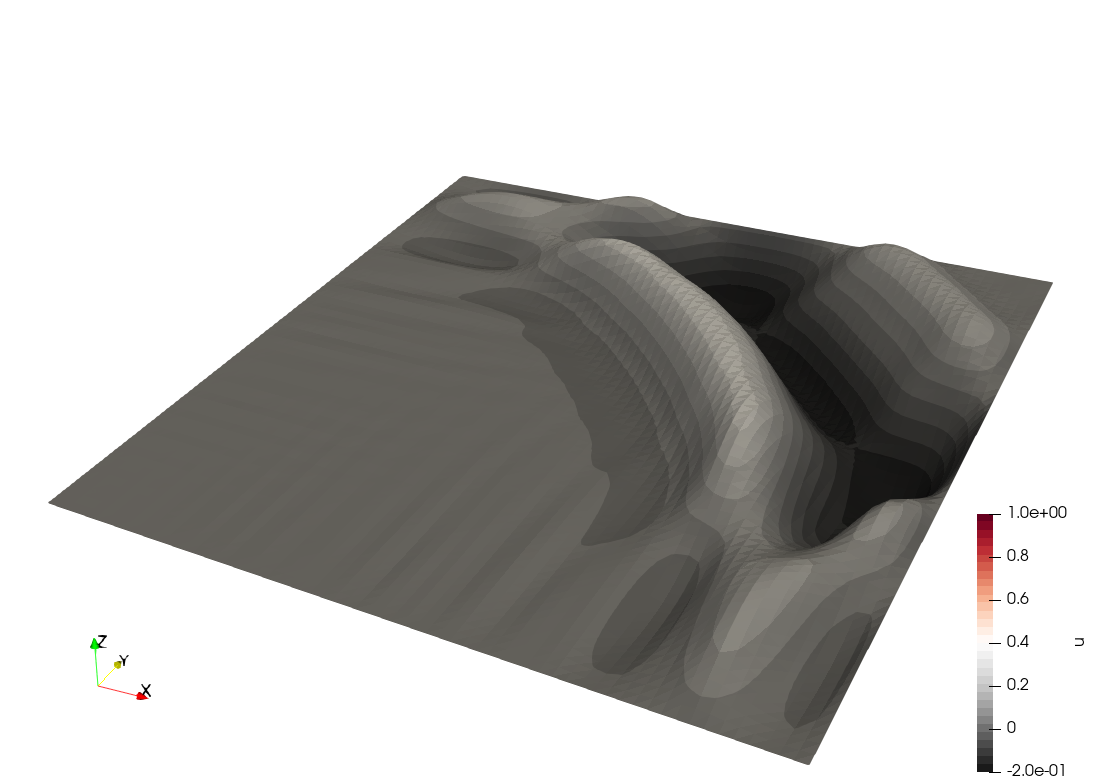
\includegraphics[width=4cm]{python_codes/fieldstone_165/results2/uuu0200.png}
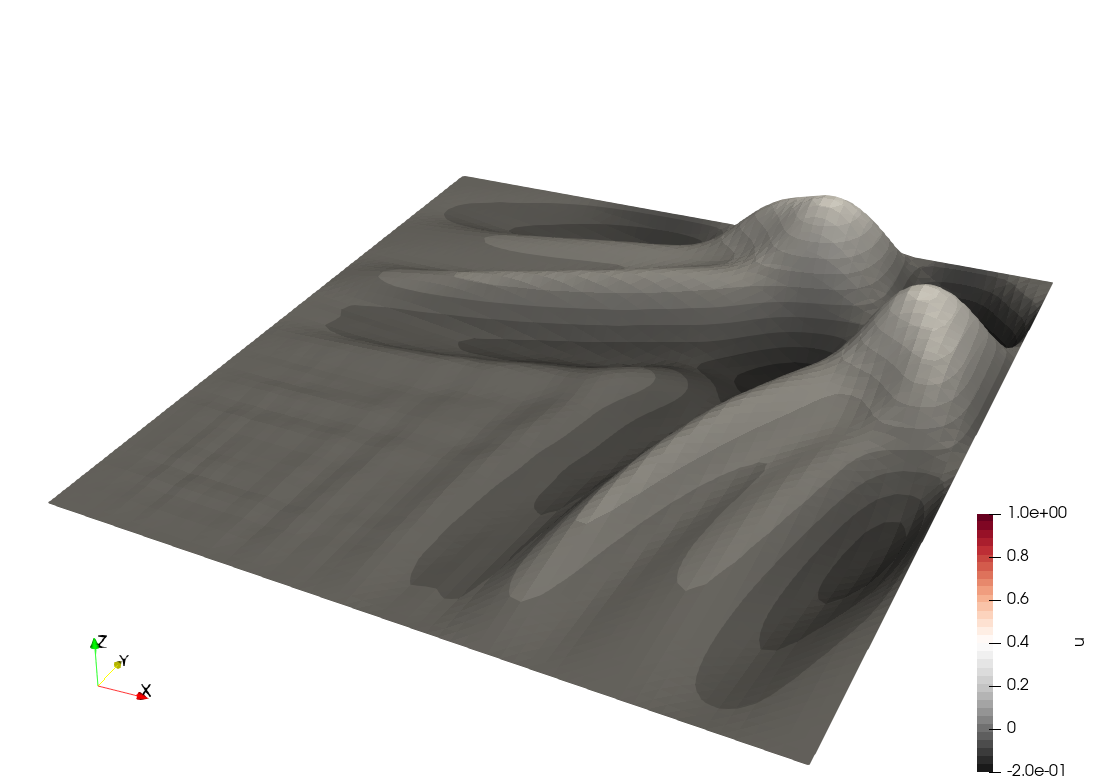
\includegraphics[width=4cm]{python_codes/fieldstone_165/results2/uuu0250.png}
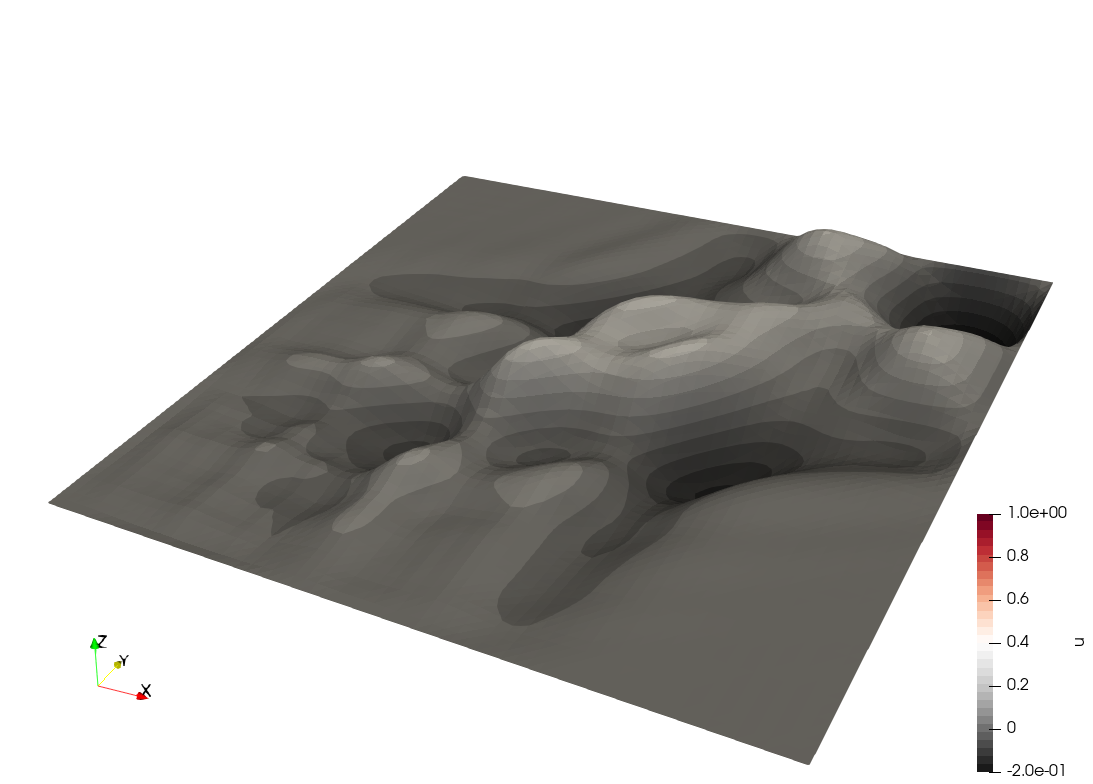
\includegraphics[width=4cm]{python_codes/fieldstone_165/results2/uuu0299.png}
\end{center}


%==============================================
\section*{Results (Experiment \# 3)}

\begin{center}
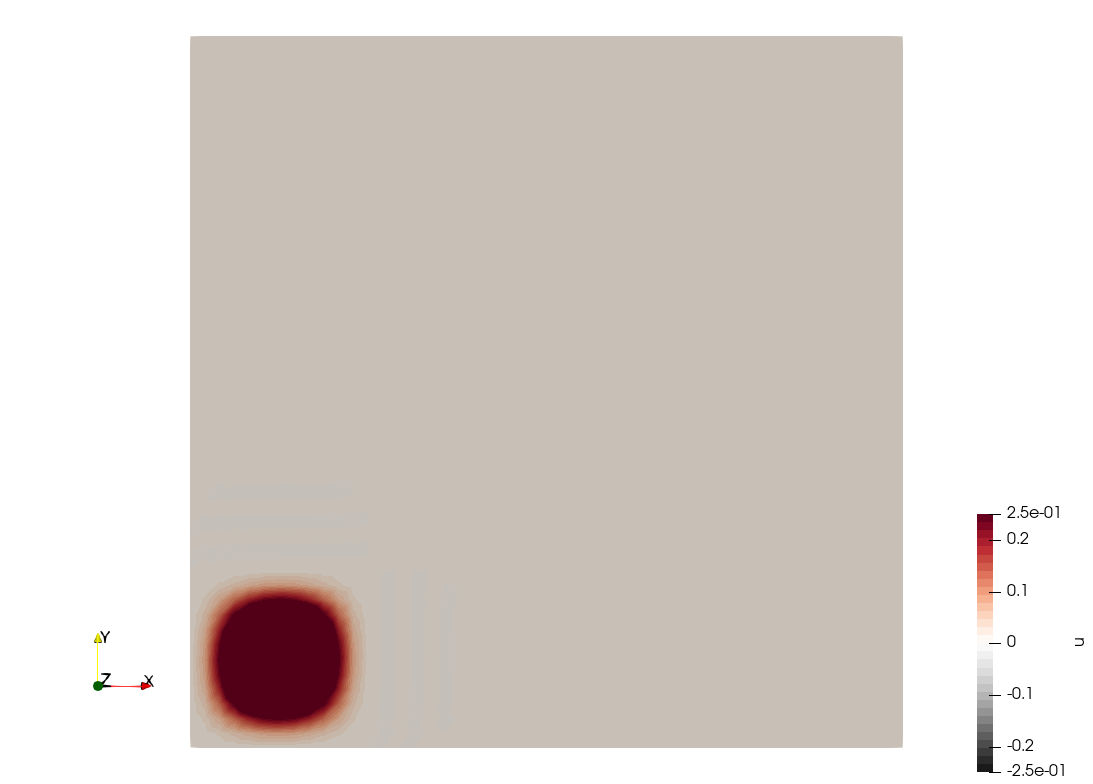
\includegraphics[width=5cm]{python_codes/fieldstone_165/results3/uu0000.png}
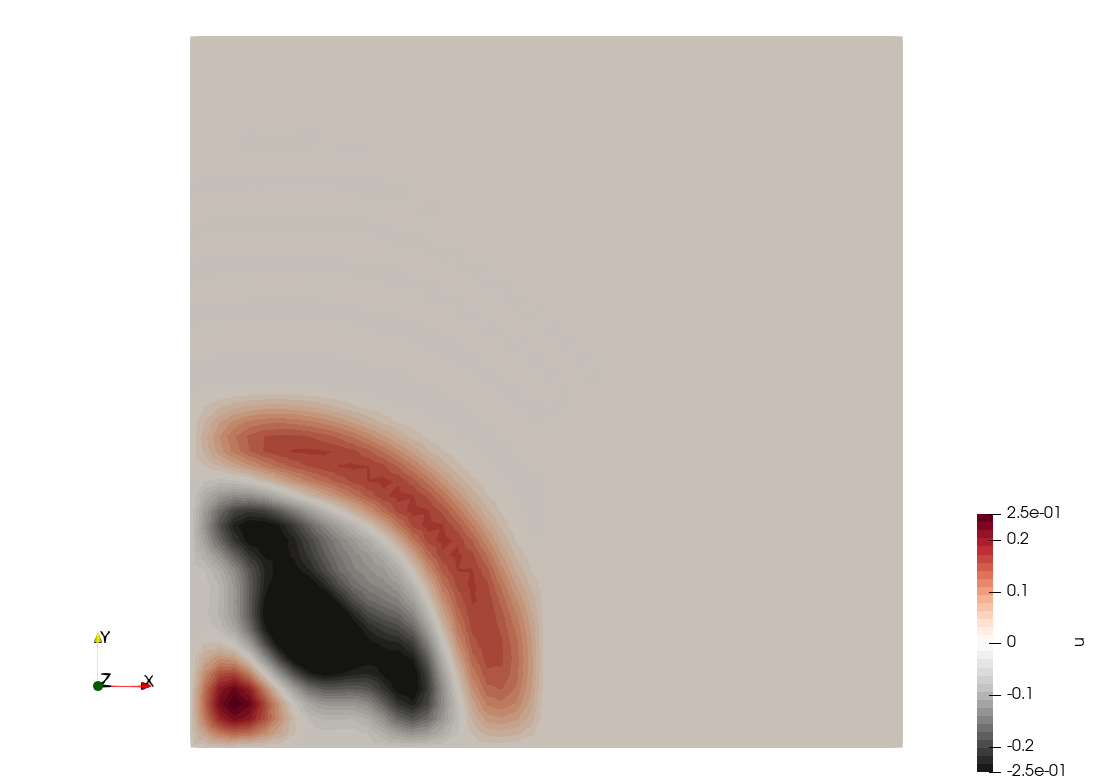
\includegraphics[width=5cm]{python_codes/fieldstone_165/results3/uu0025.png}
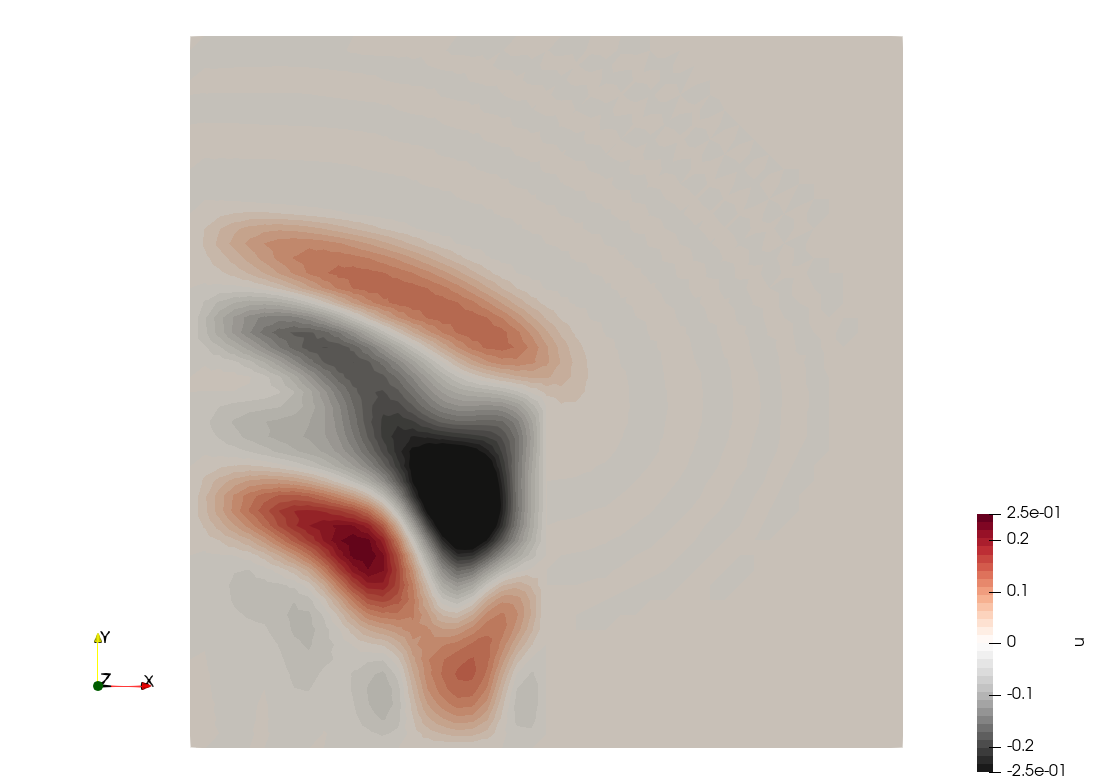
\includegraphics[width=5cm]{python_codes/fieldstone_165/results3/uu0050.png}\\
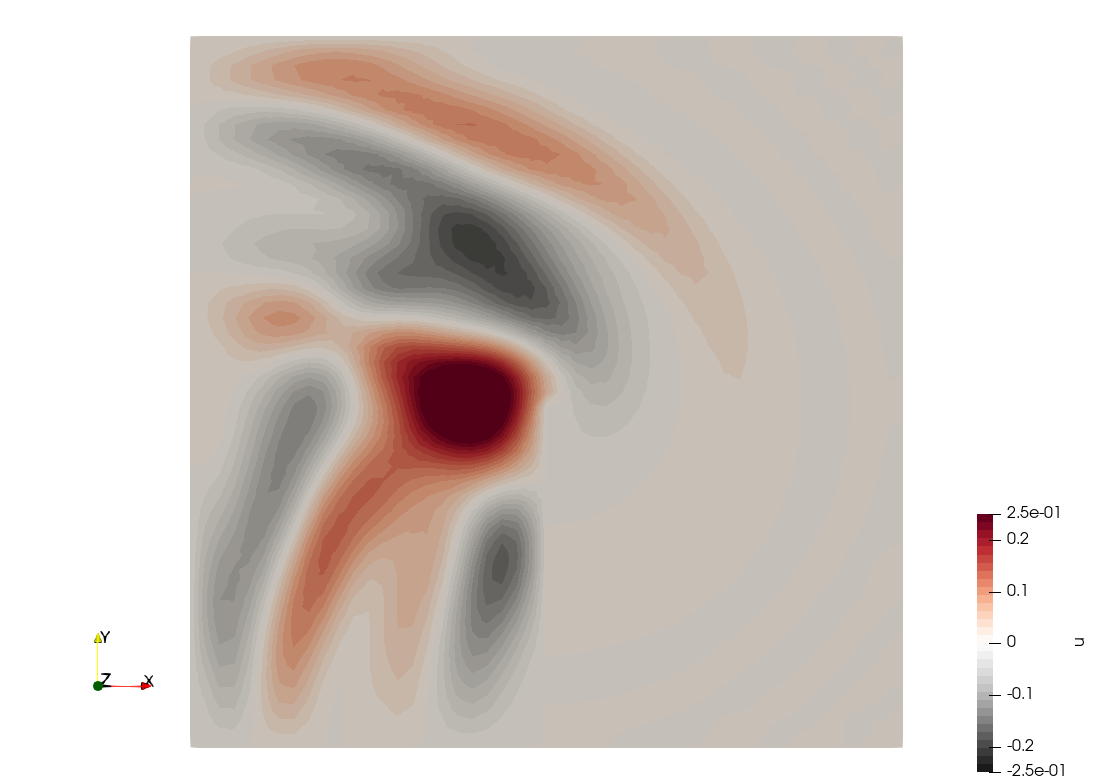
\includegraphics[width=5cm]{python_codes/fieldstone_165/results3/uu0075.png}
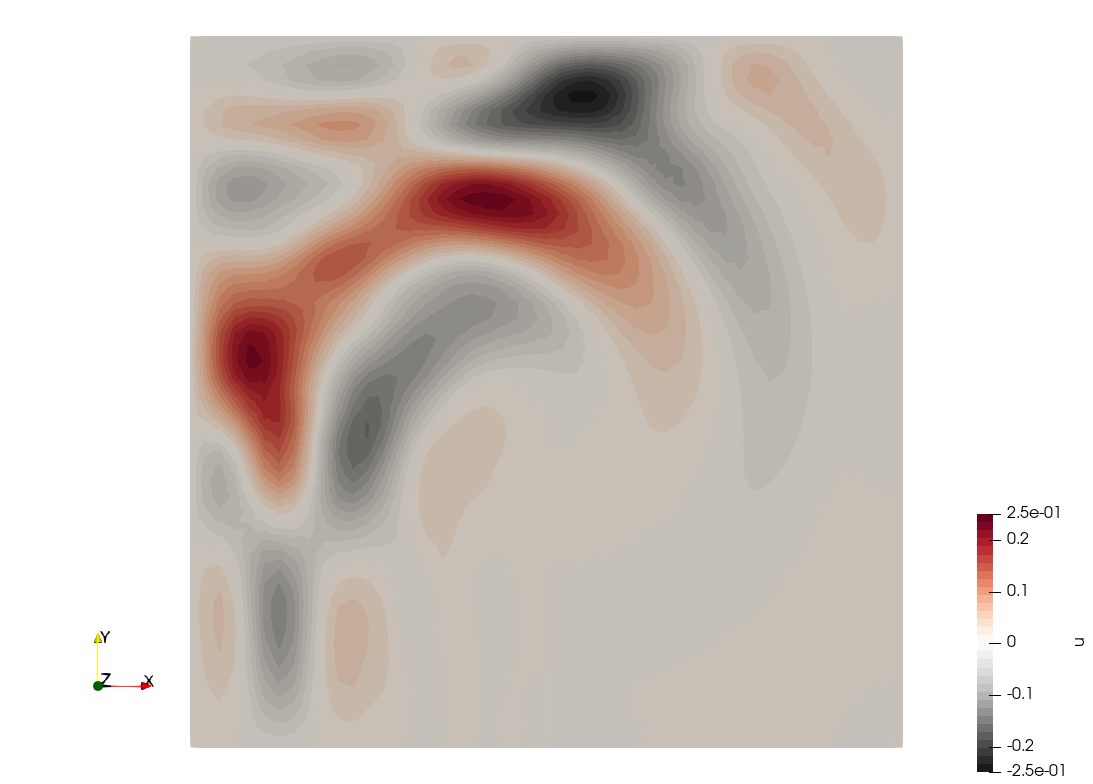
\includegraphics[width=5cm]{python_codes/fieldstone_165/results3/uu0100.png}
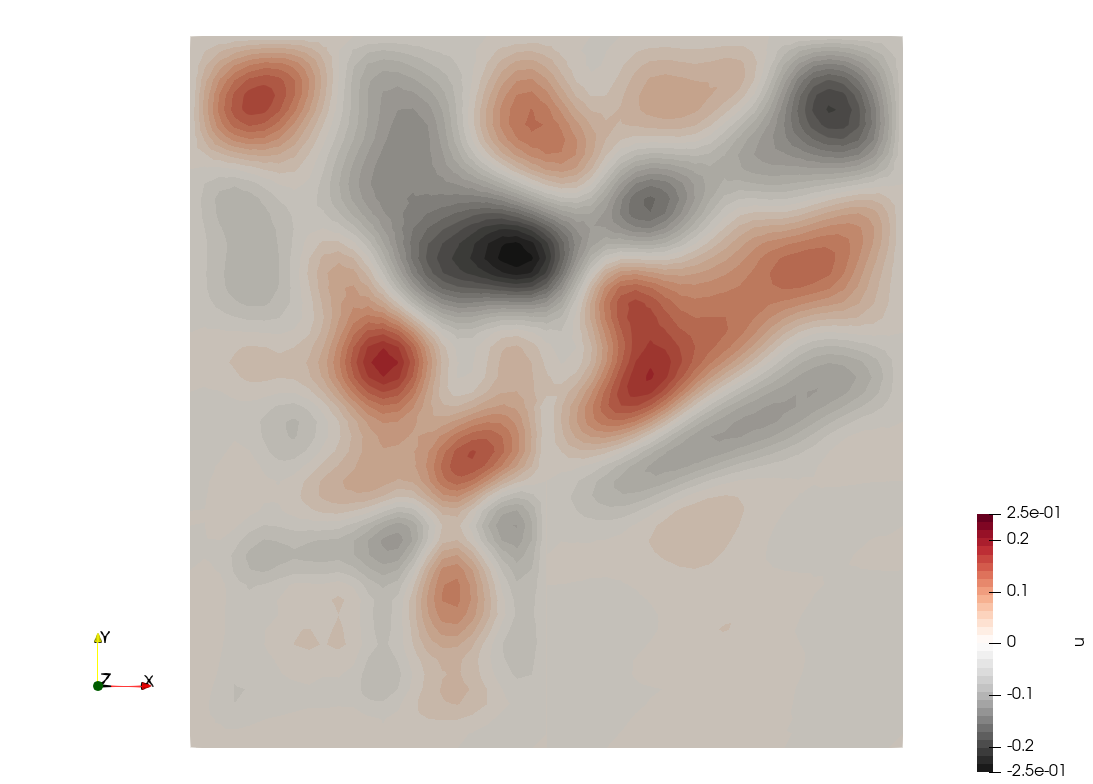
\includegraphics[width=5cm]{python_codes/fieldstone_165/results3/uu0150.png}
\end{center}





